\chapter{Bayesian Identification of Sato Tate Groups}\label{ch:12}

When Fit\'e, Kedlaya, Rotger and Sutherland classified the Sato Tate groups of abelian surfaces they did two things at once: they proved that exactly $52$ compact groups occur, up to conjugacy in $\USp(4)$, as Sato Tate groups of abelian surfaces over number fields, and they matched curves to groups by comparing empirical moments of the normalised $L$ polynomial coefficients with the moments of each candidate \cite{fkrs2012}. The second activity is statistical inference, though it is rarely described that way. This chapter makes the inference explicit: the data are the normalised traces $x_p$, the parameter is a compact group $G$, and the model is the image of Haar measure on $G$ under the trace. Bayes factors computed from this working model are consistent, with rates given by Kullback Leibler divergences, as a deterministic theorem about the actual traces whenever they are equidistributed for the true law, atoms included, and that law has finite divergence from a candidate (Theorem~\ref{thm:12consist}). We test the procedure on three genus $2$ curves, one of which lies outside the candidate set, and use that failure to argue for the full $52$ group likelihood.

\section{The inference problem}

Let $A/\Q$ be an abelian variety of dimension $g$ with good reduction outside $N$. For $p\nmid N$ the normalised Frobenius $s_p$ is a conjugacy class of the Sato Tate group $G=\mathrm{ST}(A)\subset\USp(2g)$, and the general Sato Tate conjecture (Conjecture~\ref{conj:ch3gst}) asserts that $(s_p)$ is equidistributed for the image $\mu_G$ of Haar measure. We observe $x_p=a_p/\sqrt p=\tr s_p\in[-2g,2g]$. Given $x_{p_1},\dots,x_{p_n}$, which $G$?\index{Sato Tate group}

For elliptic curves ($\SU(2)$ or $N(\mathrm{U}(1))$) complex multiplication is cheap to detect directly, but the statistical answer is the template for higher genus, where the candidates are many.

\section{Exchangeability as a working model}

The traces are determined by the curve, so a likelihood for them is a working model.\index{exchangeability} By de Finetti's theorem \cite{definetti1937,hewittsavage1955} an infinite exchangeable sequence is a mixture of independent and identically distributed sequences, so to model $(x_p)$ as exchangeable is to model it as an independent sample from an unknown law with a prior on that law. Here the prior is supported on the finitely many laws $\mu_G$, and the posterior over $G$ is the posterior over the de Finetti measure. A frequentist reading of the same likelihood is a working model in the same sense.

The only property of independent sampling used by the first order asymptotics of Bayes factors, their exponential rates, is the strong law of large numbers for the log likelihood ratio. For arithmetic data it is replaced by equidistribution, $n^{-1}\sum_{k\le n}\varphi(x_{p_k})\to\int\varphi\,d\mu_G$ for continuous $\varphi$, which plays the role of the ergodic theorem. It does not supply independence, so finite sample error probabilities are calibrated only insofar as the traces fluctuate like random ones, as Chapter~\ref{ch:05} suggests they do. Proposition~\ref{prop:01limits} gives the limitation: equidistribution is blind to alterations on sets of density zero, and so is every limit in this chapter.

\section{A general consistency theorem}

Fix a compact set $K\subset\R$, a finite set $D\subset K$, and the reference measure $\nu$ equal to Lebesgue measure on $K$ plus counting measure on $D$. Candidate laws $P_0,P_1$ and the true law $\mu_0$ have $\nu$ densities $f_0,f_1,m$, so their atoms lie in $D$. Write $h=\log(f_1/f_0)$, with values in $[-\infty,\infty]$, and for a clipping level $M>0$ write $h_M=\max(-M,\min(M,h))$. For a deterministic sequence $(x_k)$ in $K$ define the clipped log Bayes factor
\[
\log B_n^M=\sum_{k\le n}h_M(x_k).
\]
We say that $(x_k)$ is \emph{equidistributed for $\mu_0$ relative to $D$} if $n^{-1}\#\{k\le n:x_k=a\}\to\mu_0(\{a\})$ for each $a\in D$ and $n^{-1}\sum_{k\le n,\,x_k\notin D}\delta_{x_k}$ converges weakly to the restriction of $\mu_0$ to $K\setminus D$. When $\mu_0$ has no atoms this follows from equidistribution by the portmanteau theorem.

\begin{theorem}[Consistency under equidistribution; this book]\label{thm:12consist}
Suppose $(x_k)$ is equidistributed for $\mu_0$ relative to $D$, that $h$ is finite on $D$, that on $K\setminus D$ the function $h$ agrees almost everywhere with a continuous map $\tilde h:K\to[-\infty,\infty]$, through which $h$ is evaluated off $D$, and that $\mathrm{KL}(\mu_0\|P_0)<\infty$. Then for every $M$,
\[
\lim_{n\to\infty}\frac1n\log B_n^M=\int h_M\,d\mu_0,
\]
and as $M\to\infty$ the right side tends to
\[
\int h\,d\mu_0=\mathrm{KL}(\mu_0\|P_0)-\mathrm{KL}(\mu_0\|P_1)\in[-\infty,\infty).
\]
In particular, if $\mu_0=P_0$ the double limit is $-\mathrm{KL}(P_0\|P_1)$.
\end{theorem}

\begin{proof}
Divide by $n$ and split the sum according to whether $x_k\in D$. The first part is
\[
\sum_{a\in D}h_M(a)\,\frac{\#\{k\le n:x_k=a\}}n\longrightarrow\sum_{a\in D}h_M(a)\,\mu_0(\{a\}).
\]
On the second part $h_M=\tilde h_M$, a bounded continuous function on $K$, so weak convergence gives the limit $\int_{K\setminus D}\tilde h_M\,d\mu_0=\int_{K\setminus D}h_M\,d\mu_0$. Adding proves the first claim.

For the second, write $h_M=\min(h^+,M)-\min(h^-,M)$; by monotone convergence the integrals increase to those of $h^\pm$, and it suffices that $\int h^+d\mu_0<\infty$. Since $\mathrm{KL}(\mu_0\|P_0)<\infty$, $f_0>0$ almost everywhere for $\mu_0$, and on $\{m>0\}$ we have $h=\log(f_1/m)+\log(m/f_0)$. Since $\log y\le y$,
\[
\int\Bigl(\log\frac{f_1}{m}\Bigr)^+d\mu_0\le\int f_1\,d\nu=1,\qquad\int\Bigl(\log\frac{m}{f_0}\Bigr)^-d\mu_0\le\int f_0\,d\nu=1,
\]
so $\int|\log(m/f_0)|\,d\mu_0\le\mathrm{KL}(\mu_0\|P_0)+2<\infty$. Hence $h^+$ is integrable and $\int h\,d\mu_0=-\mathrm{KL}(\mu_0\|P_1)+\mathrm{KL}(\mu_0\|P_0)$.
\end{proof}

When the truth is one of the two candidates the rate is a single divergence, up to sign; in general it is a difference of two, as in the case without complex multiplication below, where $\mu_0=\ST$ is not the candidate $M_{\mathrm{ST}}$. Clipping lets weak convergence act on $h$, which may be unbounded; the independent version in Appendix~\ref{app:A} rests on the strong law of large numbers and needs no clipping.\index{Bayes factor}\index{Kullback Leibler divergence}

\section{Elliptic curves: the constants}

With $D=\{0\}$ the models are $M_{\mathrm{ST}}:x_p\sim(1-\varepsilon)\ST+\varepsilon\delta_0$ and $M_{\mathrm{CM}}:x_p\sim\mu_{\mathrm{CM}}=\frac12\delta_0+\frac12\,\mathrm{arcsine}$, where the arcsine law on $[-2,2]$ has density $(\pi\sqrt{4-x^2})^{-1}$. The small atom $\varepsilon$ keeps a single supersingular prime from being decisive; curves without complex multiplication have infinitely many of them \cite{elkies1987}. The log likelihood ratio of $M_{\mathrm{CM}}$ to $M_{\mathrm{ST}}$ is
\[
h(x)=-\log(1-\varepsilon)-\log(4-x^2)\quad(x\neq0),\qquad h(0)=\log\frac1{2\varepsilon},
\]
since $\frac12(\pi\sqrt{4-x^2})^{-1}$ divided by $(1-\varepsilon)(2\pi)^{-1}\sqrt{4-x^2}$ is $((1-\varepsilon)(4-x^2))^{-1}$. Off $D$ it extends continuously to $[-2,2]$ with values in $(-\infty,\infty]$.

\begin{lemma}\label{thm:12integral}
$\int_0^\pi\sin^2\theta\log\sin\theta\,d\theta=\frac\pi4(1-2\log2)$. Consequently
\[
\int\log(4-x^2)\,d\ST=1,\qquad \int_{-2}^2\log(4-x^2)\,\frac{dx}{\pi\sqrt{4-x^2}}=0.
\]
\end{lemma}

\begin{proof}
On $(0,\pi)$, $\log\sin\theta=-\log2-\sum_{k\ge1}k^{-1}\cos2k\theta$, with convergence in $L^2$. Multiply by $\sin^2\theta=\frac12(1-\cos2\theta)$ and integrate: $\int_0^\pi\cos2k\theta\,d\theta=0$ and $\int_0^\pi\cos2\theta\cos2k\theta\,d\theta=\frac\pi2$ if $k=1$ and $0$ otherwise. The constant term contributes $-\frac\pi2\log2$ and the $k=1$ term contributes $\frac\pi4$, which gives the first formula. With $x=2\cos\theta$ we have $\log(4-x^2)=\log4+2\log\sin\theta$, and $\ST$ becomes $\frac2\pi\sin^2\theta\,d\theta$ on $[0,\pi]$, so $\int\log(4-x^2)\,d\ST=\log4+\frac4\pi\cdot\frac\pi4(1-2\log2)=1$. Under the arcsine law $\theta$ is uniform and the constant term alone survives: $\log4+\frac2\pi(-\pi\log2)=0$.
\end{proof}

\begin{corollary}[Rates for elliptic curves; this book]\label{thm:12elliptic}
Let $E/\Q$ be an elliptic curve and $0<\varepsilon<\frac12$. If $E$ has no complex multiplication, $\lim_M\lim_n n^{-1}\log B_n^M=-1-\log(1-\varepsilon)$. If $E$ has complex multiplication, the limit is $\frac12\log\frac1{2\varepsilon}-\frac12\log(1-\varepsilon)>0$.
\end{corollary}

\begin{proof}
Without complex multiplication $(x_p)$ is $\ST$ equidistributed by Theorem~\ref{thm:04STthm}, hence equidistributed for $\ST$ relative to $\{0\}$. Apply Theorem~\ref{thm:12consist} with $\mu_0=\ST$, $P_0=M_{\mathrm{ST}}$ and $P_1=\mu_{\mathrm{CM}}$: here $\mathrm{KL}(\ST\|M_{\mathrm{ST}})=-\log(1-\varepsilon)$, and $\mathrm{KL}(\ST\|\mu_{\mathrm{CM}})=\int\log(4-x^2)\,d\ST=1$ by Lemma~\ref{thm:12integral}. With complex multiplication, $(x_p)$ is equidistributed for $\mu_{\mathrm{CM}}$ (Section~\ref{sec:04cm}), and relative to $\{0\}$, because $a_p=0$ at the good primes inert in the CM field, which have density $\frac12$, while $a_p\neq0$ at the split primes of good reduction, which are ordinary. Now $\mu_0=P_1$, and by the arcsine half of Lemma~\ref{thm:12integral} the limit is
\[
\mathrm{KL}(\mu_{\mathrm{CM}}\|M_{\mathrm{ST}})=\frac12\log\frac{1/2}{\varepsilon}+\frac12\bigl(-\log(1-\varepsilon)-0\bigr).\qedhere
\]
\end{proof}

With $\varepsilon=10^{-3}$ and $M=20$ the theoretical rates are $-0.999$ and $3.108$ nats per prime. For $E_1:y^2=x^3+x+1$ (conductor $496$, no complex multiplication) and $E_2:y^2=x^3-x$ (complex multiplication by $\Z[i]$) over the good primes below $40000$ we observed $-0.979$ and $3.102$; after only $50$ primes $\log B=-15.9$ and $+160.4$ respectively (Figure~\ref{fig:12bayes}). The slow start for $E_1$ comes from its supersingular primes $3$, $17$, $179$ and $227$ among the first $50$, each of which adds $\log(1/(2\varepsilon))=6.21$ instead of about $-1$. The CM decision is faster because half the primes give $a_p=0$, which $M_{\mathrm{ST}}$ scores as probability $\varepsilon$.

\begin{figure}[htbp]\centering
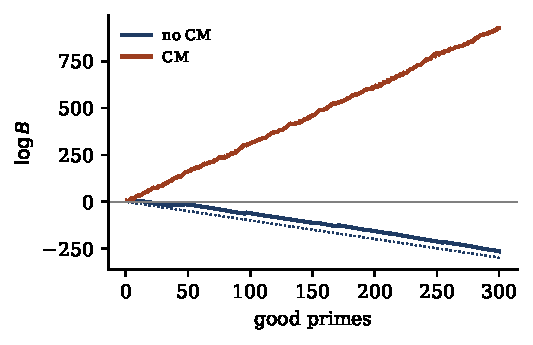
\includegraphics[width=0.62\textwidth]{figs/bayes.pdf}
\caption{Log Bayes factor of $M_{\mathrm{CM}}$ against $M_{\mathrm{ST}}$ over the first $300$ good primes for $E_1:y^2=x^3+x+1$ (no complex multiplication) and $E_2:y^2=x^3-x$ (complex multiplication), with $\varepsilon=10^{-3}$ and clipping at $M=20$. Dotted lines: the limiting slopes $-0.999$ and $3.108$ of Corollary~\ref{thm:12elliptic}.}\label{fig:12bayes}
\end{figure}

\section{Sequential testing}

Wald's sequential probability ratio test \cite{wald1947} of $P_0$ against $P_1$ stops when $\log B_n$ leaves the interval
\[
\Bigl(\log\frac{\beta}{1-\alpha},\ \log\frac{1-\beta}{\alpha}\Bigr),
\]
where $\alpha$ and $\beta$ are the target probabilities of rejecting $P_0$ when it holds and of accepting it when $P_1$ holds.\index{sequential probability ratio test} For independent observations Wald and Wolfowitz proved that no test whose error probabilities are at most those of the sequential probability ratio test has a smaller expected sample size under either hypothesis \cite{waldwolfowitz1948}, and Wald's identity, ignoring overshoot, gives $\E_1[N]\approx\log(1/\alpha)/\mathrm{KL}(P_1\|P_0)$ for small $\alpha,\beta$. By Theorem~\ref{thm:12consist} the arithmetic walk $\log B_n$ drifts at the rate computed there, so the same count, with that rate in place of the divergence, describes the actual traces as $\alpha,\beta\to0$; the error probabilities themselves come only from the working model. With $\alpha=\beta=10^{-6}$ and the rates of Corollary~\ref{thm:12elliptic}, the count is $13.8$ primes without complex multiplication and $4.4$ with it; on the actual traces the test stops at the $29$th good prime for $E_1$, delayed by the supersingular primes $3$ and $17$, and at the $4$th for $E_2$. In genus $2$ the divergences of Table~\ref{tab:12kl} are as small as $0.117$, and the approximation asks for about $120$ primes.

\section{Moments versus likelihood}

Moments are linear combinations of the Weyl averages
\[
W_\rho(n)=\frac1n\sum_{k\le n}\chi_\rho(s_{p_k}),
\]
with $\rho$ running over the irreducible representations of $\USp(2g)$, and the vector $(\int\chi_\rho\,d\mu_G)_\rho$ is the Weyl fingerprint of $G$.\index{Weyl fingerprint} If the log likelihood ratio has a uniformly convergent Peter Weyl expansion $h=\sum_\rho c_\rho\chi_\rho$, then
\[
\frac1n\log B_n=\sum_\rho c_\rho\,W_\rho(n).
\]
The log Bayes factor is a linear functional of the Weyl averages, so the vector of Weyl averages is sufficient in the limit: sequences with the same limiting fingerprint have the same Bayes factor rates for every pair of candidates. The likelihood chooses the weights $c_\rho$ optimally (Neyman Pearson); matching a few moments is valid but inefficient. In genus $2$ the conjugacy class of $s_p$ in $\USp(4)$ is determined by the normalised coefficients $(a_1,a_2)$ of the $L$ polynomial, and the trace $a_1$ alone loses information: the $55$ candidate groups of \cite{fkrs2012}, of which $52$ occur, give only $37$ distinct laws of $a_1$, while the laws of $a_1$ and of $a_2$ together distinguish all of them. No trace likelihood separates two groups with the same law of $a_1$.

\section{Genus two: three connected candidates}

We compare three connected groups through their trace laws on $[-4,4]$. Write $s(x)=(2\pi)^{-1}\sqrt{4-x^2}$ for the semicircle density.

\begin{proposition}[Weyl integration on $\USp(4)$]\label{thm:12usp4}
A class function $\varphi$ on $\USp(4)$, written in terms of the eigenvalue angles $e^{\pm i\theta_1},e^{\pm i\theta_2}$, satisfies, for the Haar probability measure $dh$,
\[
\int_{\USp(4)}\varphi\,dh=\frac8{\pi^2}\int_{[0,\pi]^2}\varphi\,(\cos\theta_1-\cos\theta_2)^2\sin^2\theta_1\sin^2\theta_2\,d\theta_1\,d\theta_2 .
\]
So $x_i=2\cos\theta_i$ have joint density $\frac12(x_1-x_2)^2s(x_1)s(x_2)$, and $t=x_1+x_2$ has density
\[
f_{\USp(4)}(t)=\frac12\int(2x-t)^2s(x)s(t-x)\,dx,\qquad f_{\USp(4)}(0)=\frac{64}{15\pi^2},
\]
with even moments $1,3,14$.
\end{proposition}

\begin{proof}
The first display is the case $g=2$ of the density \eqref{eq:ch6usp}, a consequence of Theorem~\ref{thm:ch6weyl}; its constant is $2^4/(2!\,\pi^2)=8/\pi^2$. The change of variables uses $s(x)\,dx=\frac2\pi\sin^2\theta\,d\theta$ and $(x_1-x_2)^2=4(\cos\theta_1-\cos\theta_2)^2$. At $t=0$,
\[
f(0)=2\int x^2s(x)^2\,dx=\frac{1}{2\pi^2}\int_{-2}^2(4x^2-x^4)\,dx=\frac{64}{15\pi^2},
\]
and, for independent semicircular $x_1,x_2$,
\[
\E_{\USp(4)}t^2=\tfrac12\E\bigl[(x_1+x_2)^2(x_1-x_2)^2\bigr]=\E x_1^4-(\E x_1^2)^2=1;
\]
the other moments are similar.
\end{proof}

The second candidate, $\SU(2)\times\SU(2)$ embedded block diagonally, has trace density $s*s$ (value $8/(3\pi^2)$ at $0$, moments $2,10,70$). For a genus $2$ curve $C$ over $\Q$ it arises exactly when all endomorphisms of $\mathrm{Jac}(C)_{\overline\Q}$ are defined over $\Q$ and $\mathrm{End}(\mathrm{Jac}(C)_{\overline\Q})\otimes\R\simeq\R\times\R$ \cite{fkrs2012}, for instance when $\mathrm{Jac}(C)$ is isogenous over $\Q$ to a product of two elliptic curves without complex multiplication that are not isogenous over $\overline\Q$. The third, $\SU(2)$ embedded diagonally, has trace $2x$ with $x$ semicircular, density $(8\pi)^{-1}\sqrt{16-t^2}$ and moments $4,32,320$; it arises exactly when the same holds with $M_2(\R)$ in place of $\R\times\R$, for instance when $\mathrm{Jac}(C)$ is isogenous over $\Q$ to the square of an elliptic curve without complex multiplication.

Table~\ref{tab:12kl} gives the divergences, computed by quadrature of the convolution integrals and confirmed by Monte Carlo. Near $\pm4$ the $\USp(4)$ density vanishes like $(4-|t|)^4$, the diagonal density only like $(4-|t|)^{1/2}$, so the log likelihood ratio of the diagonal group against $\USp(4)$ is large where the diagonal law still puts appreciable mass, and $\mathrm{KL}(\text{diag}\|\USp(4))=1.061$ is more than twice its reverse $0.456$.

\begin{table}[htbp]\centering\small
\begin{tabular}{lccc}
\toprule
$P\setminus Q$ & $\USp(4)$ & $\SU(2)\times\SU(2)$ & diagonal\\
\midrule
$\USp(4)$ & 0 & 0.117 & 0.456\\
$\SU(2)\times\SU(2)$ & 0.168 & 0 & 0.161\\
$\SU(2)$ diagonal & 1.061 & 0.262 & 0\\
\bottomrule
\end{tabular}
\caption{Kullback Leibler divergences $\mathrm{KL}(P\|Q)$ in nats between the trace laws of three connected Sato Tate groups in genus $2$, with $P$ indexing rows and $Q$ columns. They are the per prime error exponents of Theorem~\ref{thm:12consist}.}\label{tab:12kl}
\end{table}

\section{Three curves}

We counted points on three genus $2$ curves at all odd primes below $10^5$ that do not divide the discriminant of the defining polynomial ($9589$ or $9590$ primes per curve), and computed posteriors with a uniform prior, likelihoods from the trace densities above and clipping at $20$ (Figures~\ref{fig:12genus2} and \ref{fig:12posterior}).

$C_1:y^2=x^5-x+1$. The quintic has Galois group $S_5$, so by a theorem of Zarhin \cite{zarhin2000} the Jacobian has no endomorphisms over $\overline\Q$ beyond $\Z$, and its group is $\USp(4)$. The even moments $1.020,3.166,15.40$ are within about two standard errors of the $\USp(4)$ values $1,3,14$. The posterior probability of $\USp(4)$ is $0.426$ after $10$ primes, $0.984$ after $50$ and $0.99998$ after $100$. The per prime log Bayes factor of $\SU(2)\times\SU(2)$ against $\USp(4)$ is $-0.111$, against the theoretical $-0.117$, and that of the diagonal group is $-0.447$, against $-0.456$. For $C_1$ the theorem is conditional on the general Sato Tate conjecture.

$C_2:y^2=x^6+3x^4+x^2+1$. The involutions $(x,y)\mapsto(-x,\pm y)$ split the Jacobian over $\Q$, up to isogeny, into $E:y^2=x^3-2x+2$ and $E':y^2=x^3+x^2+3x+1$, so $a_p(C_2)=a_p(E)+a_p(E')$. Their $j$ invariants $-13824/19$ and $32768/19$ are not integers, so neither has complex multiplication. Curves without complex multiplication that are isogenous over $\overline\Q$ are, over $\Q$, isogenous up to a quadratic twist, which would force $|a_5(E)|=|a_5(E')|$; since $a_5(E)=1$ and $a_5(E')=-3$, $E$ and $E'$ are not isogenous over $\overline\Q$. The group is therefore $\SU(2)\times\SU(2)$, and by the joint Sato Tate theorem (Theorem~\ref{thm:04joint}) the limits for $C_2$ hold unconditionally. The moments $1.999,9.91,68.3$ match this group, its posterior is $0.998$ after $50$ primes, and the per prime rate against $\USp(4)$ is $0.167$, against the theoretical $0.168$.

$C_3:y^2=x^6+x^3+1$. The moments $1.98,15.8,158.8$ fit none of the candidates. The reason is visible in the data: $a_p=0$ for every prime $p\equiv2\bmod3$ and for no prime $p\equiv1\bmod3$ in our range, so the trace law has an atom of mass $0.501$ at $0$, and on the remaining primes the even moments $3.96,31.7,318$ are close to $4,32,320$. This suggests a disconnected group with identity component $\SU(2)$ diagonal; among the $55$ groups of \cite{fkrs2012} exactly two, denoted $E_2$ and $J(E_1)$ there, have trace moments $2,16,160$, and only the law of $a_2$ separates them. The curve has extra automorphisms, $(x,y)\mapsto(\zeta_3x,y)$ and $(x,y)\mapsto(1/x,y/x^3)$, and its group lies outside our candidate set.

\begin{figure}[htbp]\centering
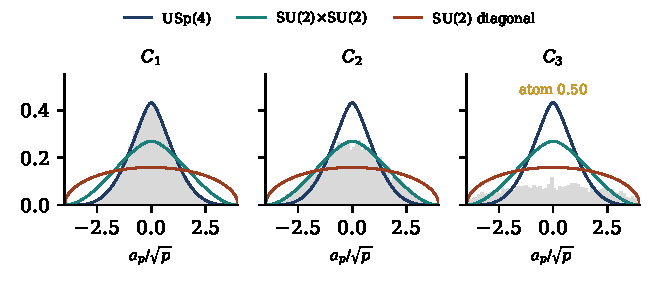
\includegraphics[width=0.92\textwidth]{figs/genus2.pdf}
\caption{Histograms of $a_p/\sqrt p$ for $C_1$, $C_2$ and $C_3$ at the good primes $p<10^5$, against the trace densities of $\USp(4)$, $\SU(2)\times\SU(2)$ and $\SU(2)$ diagonal. For $C_3$ the histogram shows the primes with $a_p\neq0$, scaled to total mass $0.50$; the atom at $0$ carries the rest.}\label{fig:12genus2}
\end{figure}

\begin{figure}[htbp]\centering
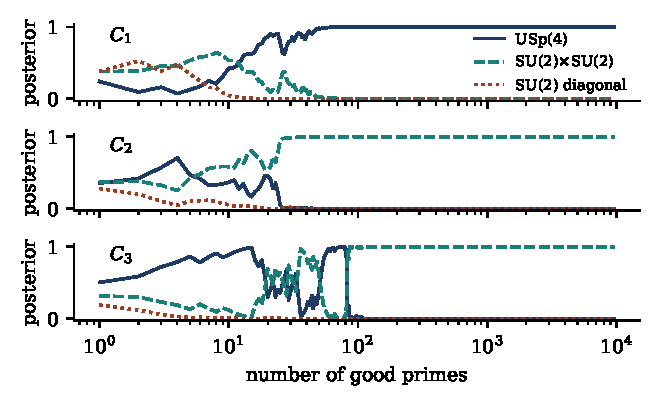
\includegraphics[width=0.78\textwidth]{figs/ch12_posterior.pdf}
\caption{Posterior probabilities of $\USp(4)$, $\SU(2)\times\SU(2)$ and $\SU(2)$ diagonal for $C_1$, $C_2$ and $C_3$ against the number of good primes (logarithmic scale), uniform prior. For $C_3$, whose group is not a candidate, the posterior settles on $\SU(2)\times\SU(2)$ after about $100$ primes.}\label{fig:12posterior}
\end{figure}

\section{Misspecification}

Berk \cite{berk1966} showed that when the true law $\mu_0$ is outside a parametric model, the posterior concentrates, under regularity conditions, on the Kullback Leibler projection, the set of parameters minimising $\mathrm{KL}(\mu_0\|P_\theta)$; see \cite{kleijnvandervaart2006} for infinite dimensional models.\index{misspecification} Theorem~\ref{thm:12consist} is the deterministic form for two candidates: the rate $\mathrm{KL}(\mu_0\|P_0)-\mathrm{KL}(\mu_0\|P_1)$ favours the candidate closer to $\mu_0$.

For $C_3$ the true law $\mu_0\approx\frac12\delta_0+\frac12\,\mathrm{law}(2x)$ has an atom and every candidate is continuous, so every divergence $\mathrm{KL}(\mu_0\|\mu_G)$ is infinite and the projection is undefined. A likelihood computed from densities scores the atom by the density value at $0$, and with $f_G$ the trace density of $G$ the posterior then concentrates on the maximiser of $\frac12\log f_G(0)+\frac12\E\log f_G(2x)$, with $x$ semicircular. The values $f_G(0)$ are $0.432$, $0.270$ and $0.159$ for $\USp(4)$, $\SU(2)\times\SU(2)$ and the diagonal group, so the atom favours the peaked $\USp(4)$ density, the continuous part favours the diagonal group, and the compromise is $\SU(2)\times\SU(2)$: predicted rates against $\USp(4)$ are $0.164$ (product) and $0.031$ (diagonal), observed $0.158$ and $0.021$, and the posterior on the product exceeds $0.99$ after $100$ primes. This is an artefact of how the atom is scored.

The honest reading for $C_3$ is \emph{none of the candidates}: a posterior near one measures fit relative to the list. The moments expose the problem at once: for every candidate at least one of them is off by dozens of standard errors (for $\SU(2)\times\SU(2)$ the second moment fits, the fourth and sixth do not). The likelihood is far less sensitive: the average log likelihood under the winner is $-1.80$ per prime, against $-1.75$ expected if the traces followed the winning law, a gap of about seven standard errors after $9590$ primes. The remedy is expansion to all $52$ groups of \cite{fkrs2012}, which forces the likelihood to carry discrete components: atoms at $a_1=0$ from disconnected groups with components on which the trace vanishes identically. With Lebesgue measure plus atoms as reference, as in Theorem~\ref{thm:12consist}, the atom alone separates $C_3$ from every connected candidate: each prime $p\equiv2\bmod3$ adds $\log(1/(2\varepsilon))$ to the log Bayes factor if the connected candidates carry a small atom $\varepsilon$ at $0$, as in the elliptic case, and the clipping level $M$ if they carry none.

\section{Nonparametric alternatives and arithmetic priors}

Distrusting the candidate list, one can put a nonparametric prior on the trace law. Dirichlet process draws \cite{ferguson1973} are discrete, so against a parametric $\mu_G$ a P\'olya tree \cite{lavine1992} or a Dirichlet process mixture is more natural; the Bayes factor of $\mu_G$ against such a prior is a test of fit of $\mu_G$ itself rather than a comparison within the list. Alternatively, a prior on moment sequences through the canonical moments of Dette and Studden \cite{dettestudden1997}, free coordinates in $(0,1)$ for the moment space of $[-4,4]$, tests whether the empirical sequence lies near some fingerprint. A roughness prior in the sense of Good and Gaskins, on densities of the eigenvalue angles that vanish on the walls of the alcove, has, formally, the Sato Tate law of a simply connected group as its mode, and for $\SU(2)$ it shrinks the empirical moments of the symmetric powers towards those of that law (Theorem~\ref{thm:lapgg}). The Dirichlet process has already appeared in Chapter~\ref{ch:pd}, not as a prior but as the limit law of the normalised Frobenius labelled factorisation of a random integer, with the Haar measure of Chebotarev's theorem as its base measure.\index{Dirichlet process}

Arithmetic should inform the prior. The Sato Tate group of an abelian surface $A$ is determined by its Galois endomorphism type, the real algebra $\mathrm{End}(A_{\overline\Q})\otimes\R$ with its Galois action \cite{fkrs2012}, which can be computed rigorously \cite{cmsv2019}; in particular, the component group of the Sato Tate group is the Galois group of the smallest field over which all endomorphisms are defined. For $C_3$ the automorphism $(x,y)\mapsto(\zeta_3x,y)$ induces an endomorphism of the Jacobian that is defined over $\Q(\sqrt{-3})$ but not over $\Q$, so the group of $C_3$ is disconnected and none of the three connected candidates can be right, a fact available before any prime is examined. Once the endomorphism type is known, Frobenius data test the Sato Tate conjecture rather than estimate the group. Across a database, group frequencies among curves of bounded conductor give an empirical Bayes prior \cite{robbins1956}, dominated by $\USp(4)$.\index{empirical Bayes}

\section{Notes}

The moment method in genus $2$ goes back to Kedlaya and Sutherland \cite{kedlayasutherland2009}; the classification \cite{fkrs2012} and the survey \cite{sutherland2019} systematise it. Equidistribution is proved for many but not all of the $52$ groups, and is open for $\USp(4)$ (Chapter~\ref{ch:03}).

The core of Theorem~\ref{thm:12consist}, that the average log likelihood ratio converges to a difference of divergences, is the argument of Wald's proof that maximum likelihood is consistent \cite{wald1949}, with equidistribution in place of the strong law of large numbers; the divergence is that of Kullback and Leibler~\cite{kullbackleibler1951}. Theorem~\ref{thm:12consist} and Corollary~\ref{thm:12elliptic} are ours; they assume equidistribution and prove nothing new about Sato Tate.

\section{Exercises}

\begin{enumerate}
\item Prove $\int_0^\pi\log\sin\theta\,d\theta=-\pi\log2$ without Fourier series, by the substitution $\theta\mapsto2\theta$ and symmetry. Deduce that the arcsine mean of $\log(4-x^2)$ is $0$.
\item Show that $\mathrm{KL}(\ST\|\mu_{\mathrm{CM}})=1$ while $\mathrm{KL}(\mu_{\mathrm{CM}}\|\ST)=\infty$, and explain why the atom $\varepsilon$ is needed. Show that both limits in Corollary~\ref{thm:12elliptic} improve as $\varepsilon$ decreases, and that the price is the jump $\log(1/(2\varepsilon))$ that each supersingular prime of a curve without complex multiplication adds to $\log B_n$. For which $\varepsilon$ is the rate without complex multiplication at most $-0.99$, and what is the smallest rate with complex multiplication on that range?
\item Using Proposition~\ref{thm:12usp4}, show that the $\USp(4)$ trace has fourth moment $3$ and that $f_{\USp(4)}(t)$ vanishes like $(4-|t|)^{4}$ as $|t|\to4$. Explain the asymmetry in Table~\ref{tab:12kl}.
\item (Probabilistic.) From Wald's identity and optional stopping derive the approximation $\E_1[N]\approx\log(1/\alpha)/\mathrm{KL}(P_1\|P_0)$. Evaluate it for $\SU(2)\times\SU(2)$ against $\USp(4)$ with $\alpha=10^{-6}$.
\item For the limiting law of $C_3$ and each of the three connected candidates $G$, compute numerically
\[
\tfrac12\log f_G(0)+\tfrac12\E\log f_G(2x),\qquad x\text{ semicircular},
\]
and verify that $\SU(2)\times\SU(2)$ wins.
\item Show that altering $(x_k)$ on a set of indices of density zero leaves every limit in Theorem~\ref{thm:12consist} unchanged.
\end{enumerate}

\section{Open computational problems}

\begin{compproblem}[The group of $y^2=x^6+x^3+1$]
Objective: identify the Sato Tate group of $C_3$ among the $52$ groups of \cite{fkrs2012} from Frobenius data; its trace moments point to $E_2$ and $J(E_1)$ in the notation of \cite{fkrs2012}, which share the law of $a_1$. Data: the normalised coefficients $(a_1,a_2)$ of the $L$ polynomial at all good primes below $2^{30}$. Route: \texttt{smalljac} or average polynomial time point counting \cite{harveysutherland2014}; moments of $a_1$ and $a_2$ up to order $12$ and the frequency of $a_1=0$ by residue class mod $3$, compared with the tables of \cite{fkrs2012} and checked against the endomorphism type \cite{cmsv2019}. Deliverable: the group, its posterior against the other group with the same law of $a_1$, and the number of primes needed to reach $1-10^{-9}$. Why it matters: it completes this chapter's misspecified example and measures what $a_2$ adds.
\end{compproblem}

\begin{compproblem}[A likelihood library, a classifier and the error exponent matrix]
Objective: build the joint densities of $(a_1,a_2)$ for all $52$ groups, atoms and lower dimensional components included, as densities against a reference measure in the sense of Theorem~\ref{thm:12consist}; compute the $52\times52$ matrix of divergences $\mathrm{KL}(\mu_G\|\mu_{G'})$ for $(a_1,a_2)$ and for $a_1$ alone (infinite where $\mu_G$ charges a set that $\mu_{G'}$ does not, and zero for $a_1$ alone when two groups share its law); and run Wald's test on every genus $2$ curve in the LMFDB \cite{lmfdb} with primes up to $10^7$. Route: Weyl integration on identity components in Sage, Monte Carlo on cosets ($10^8$ draws per group), exact arithmetic on atoms. Deliverable: the library, the divergence matrix with its near ties, a confusion matrix against the LMFDB labels, and stopping times against $\log(1/\alpha)/\mathrm{KL}$. Why it matters: the divergences are the error exponents of every test, and the near ties are the hard instances. The library and the divergence matrix are the new objects here; the run to $10^7$ is a pilot for Computational Problem~3.2, which goes to $2^{30}$, and the library must reproduce the Weyl fingerprints of Computational Problem~4.2.
\end{compproblem}

\begin{compproblem}[Genus three with an empirical Bayes prior]
Objective: extend the classifier to the $410$ groups of genus $3$ \cite{fks2021}, building on Sutherland's computations. Data: plane quartics and hyperelliptic curves of genus $3$ with discriminant below $10^7$, primes up to $2^{26}$. Route: average polynomial time point counting \cite{harveysutherland2014} and a Dirichlet prior on group frequencies estimated across the database. Deliverable: frequencies, posteriors, and curves fitted by no group. Why it matters: with $410$ candidates, shared trace laws and near ties should be far more common than in genus $2$, and the experiment measures how much of the classification Frobenius data can resolve. It builds on the genus $3$ sample of Computational Problem~3.2, adding a prior estimated across the database and a search for the curves that no group fits.
\end{compproblem}
